\documentclass[11px]{article}
\usepackage{graphicx} % Required for inserting images
\usepackage{bm}
\usepackage{tikz} 
\usepackage{amsmath,amsfonts,amssymb,amsthm}
\usepackage{newpxtext} 
\usepackage{relsize}
\usepackage{comment}
\usepackage{booktabs}
\usepackage{stackengine} 
\usepackage{adjustbox}
\usepackage{mathtools}

\title{Applied math exercise 3}
\author{Erik Paskalev}
\date{September 2024}

\begin{document}

\maketitle

\section*{Exercise 3.5. \normalfont In some communication system bits like 0 and 1 are transmitted in several steps. In every step the probability that the bit stays correct, is equal to 0.8.}

\section*{\normalfont (a) Describe this communication system as a Markov process, and give its state diagram and transition matrix.}

\section*{Answer: $S_1$ means the bit is transmitted correctly. $S_2$ means the bit is transmitted incorrectly.}

\begin{center}
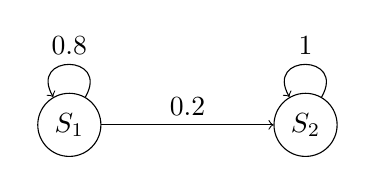
\begin{tikzpicture}[centered, node distance={30mm}, main/.style = {draw, circle}] 
\node[main] (1) {$S_1$}; 
\node[main] (2) [right of=1] {$S_2$}; 
\draw[->] (1) to [out=60, in=120, looseness=4] node[midway, above]{0.8} (1);
\draw[->] (1) to [out=0, in=180, looseness=0] node[midway, above]{0.2} (2);
\draw[->] (2) to [out=60, in=120, looseness=4] node[midway, above]{1} (2);
\end{tikzpicture}
\end{center}

\begin{equation}
P = \begin{pmatrix}
\frac{4}{5} & \frac{1}{5} \\
0 & 1 \\
\end{pmatrix}
\end{equation}

\section*{\normalfont (b) Determine the probability that the bit 0 gets received as 0 after 4 steps.}

\section*{Answer: Since the state $S_2$ is absorbing that means the only way to receive 0 after 4 steps is $S_1S_1S_1S_1$  the probability following this path is ${(0.8)}^4 = \frac{256}{625} = 0.4096$} 

\section*{Exercise 3.6. \normalfont Some mathematician travels every morning to the university and every afternoon to his house. He has one umbrella. If it is dry, he doesn't bring his umbrella with him. Otherwise he does take hise umbrella with him if possible (if for example the umbrella is at the university when he leaves home, he obviously cannot use his umbrella). The probability that it rains in the morning is 0.2, while it rains in the afternoon with probability 0.1. This situation can be described by a Markov chain. We distinguish the following four states:}

\begin{equation}
\begin{split}
& S_1: \text{ Mathematician at home, umbrella at home.} \\
& S_2: \text{ Mathematician at home, umbrella at university.} \\
& S_3: \text{ Mathematician at university, umbrella at home.} \\
& S_4: \text{ Mathematician at university, umbrella at university.} \\
\end{split}
\end{equation}

\section*{\normalfont Every trip of the mathematician corresponds to a transition between two of these states.}

\subsection*{\normalfont (a) Give the state diagram of this Markov model. Put S1 and S4 next to each other.}

\subsection*{Answer: }

\begin{center}
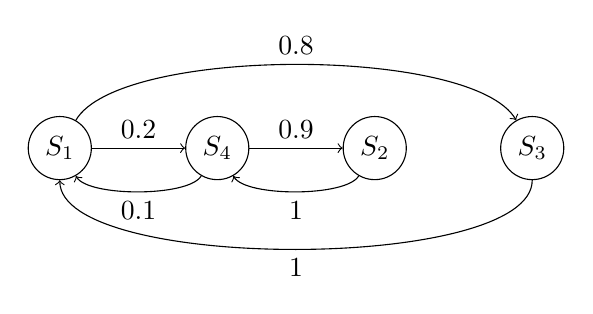
\begin{tikzpicture}[centered, node distance={20mm}, main/.style = {draw, circle}] 
\node[main] (1) {$S_1$}; 
\node[main] (4) [right of=1] {$S_4$}; 
\node[main] (2) [right of=4] {$S_2$}; 
\node[main] (3) [right of=2] {$S_3$}; 
\draw[->] (1) to node[midway, above]{0.2} (4);
\draw[->] (4) to node[midway, above]{0.9} (2);
\draw[->] (1) to [out=60, in=120, looseness=0.5] node[midway, above]{0.8} (3);
\draw[->] (4) to [out=240, in=300, looseness=0.5] node[midway, below]{0.1} (1);
\draw[->] (2) to [out=240, in=300, looseness=0.5] node[midway, below]{1} (4);
\draw[->] (3) to [out=270, in=270, looseness=0.5] node[midway, below]{1} (1);
\end{tikzpicture}
\end{center}

\subsection*{\normalfont (b) Determine the transition matrix P.}

\subsection*{Answer:}

\begin{center}
$
P = 
\begin{pmatrix}
0 & 0 & 0.8 & 0.2 \\
0 & 0 & 0 & 1 \\
1 & 0 & 0 & 0 \\
0.1 & 0.9 & 0 & 0 \\
\end{pmatrix}
$
\end{center}

\subsection*{\normalfont (c) Suppose that on some Monday evening (t = 1) both the mathematician and his umbrella are at home. Compute the probability that the mathematician and his umbrella are at home on Wednesday evening (t = 5).}

\subsection*{Answer: }

\begin{equation}
\begin{split}
P(X_5 = S_1|X_1 = S_1) & = P_{11}^{(4)} \\
P^4 = {
\begin{pmatrix}
0 & 0 & 0.8 & 0.2 \\
0 & 0 & 0 & 1 \\
1 & 0 & 0 & 0 \\
0.1 & 0.9 & 0 & 0 \\
\end{pmatrix}
}^4 & = 
\begin{pmatrix}
0.69 & 0.31 & 0 & 0 \\
0.17 & 0.83 & 0 & 0 \\
0 & 0 & 0.66 & 0.34 \\
0 & 0 & 0.14 & 0.86 \\
\end{pmatrix} \\
P_{11}^{(4)} & = 0.69
\end{split}
\end{equation}

\section*{Exercise 3.9.}

\section*{\normalfont (a) Identify the communicating classes of the following transition matrix:}

\begin{equation}
P = \begin{pmatrix}
\frac{1}{2} & 0 & 0 & 0 & \frac{1}{2} \\
0 & \frac{1}{2} & 0 & \frac{1}{2} & 0 \\
0 & 0 & 1 & 0 & 0 \\
0 & \frac{1}{4} & \frac{1}{4} & \frac{1}{4} & \frac{1}{4} \\
\frac{1}{2} & 0 & 0 & 0 & \frac{1}{2} \\
\end{pmatrix}
\end{equation}

\section*{Answer: \normalfont Based on the diagram of the Markov chain the communicating classes are $\{S_1,S_5\}, \{S_2,S_4\}, \{S_3\}$}

\begin{center}
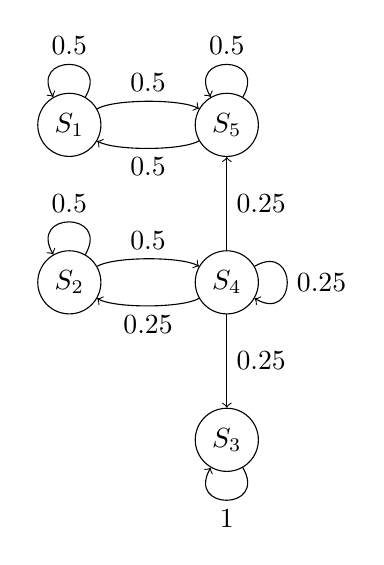
\begin{tikzpicture}[centered, node distance={20mm}, main/.style = {draw, circle}] 
\node[main] (1) {$S_1$}; 
\node[main] (5) [right of=1] {$S_5$}; 
\node[main] (2) [below of=1] {$S_2$}; 
\node[main] (4) [below of=5] {$S_4$}; 
\node[main] (3) [below of=4] {$S_3$}; 


\draw[->] (1) to [out=60, in=120, looseness=4] node[midway, above]{0.5} (1);
\draw[->] (5) to [out=60, in=120, looseness=4] node[midway, above]{0.5} (5);
\draw[->] (1) to [out=30, in=150, looseness=0.5] node[midway, above]{0.5} (5);
\draw[->] (5) to [out=210, in=330, looseness=0.5] node[midway, below]{0.5} (1);
\draw[->] (2) to [out=60, in=120, looseness=4] node[midway, above]{0.5} (2);
\draw[->] (2) to [out=30, in=150, looseness=0.5] node[midway, above]{0.5} (4);
\draw[->] (4) to [out=210, in=330, looseness=0.5] node[midway, below]{0.25} (2);
\draw[->] (4) to [out=90, in=270, looseness=0] node[midway, right]{0.25} (5);
\draw[->] (4) to [out=270, in=90, looseness=0] node[midway, right]{0.25} (3);
\draw[->] (4) to [out=30, in=330, looseness=4] node[midway, right]{0.25} (4);
\draw[->] (3) to [out=300, in=240, looseness=4] node[midway, below]{1} (3);
\end{tikzpicture}
\end{center}

\section*{\normalfont (b) Specify in each case which classes are recurrent and which are transient. Are there any absorbing states?}

\section*{Answer: \normalfont Since the class $\{S_3\}$ has no outward edges, then the class is closed. From that, we can directly conclude that $\{S_3\}$ is also recurrent and $S_3$ is absorbing. Analogously For the class $\{S_1, S_5\}$ it holds that it is closed/recurrent and both $S_1$ and $S_5$ are absorbing states. For the last class $\{S_2, S_4\}$ it is neither closed nor recurrent since there are edges that flow into closed classes, and that makes $S_2, S_4$ transient states as a result.}

\section*{Exercise 4.8. \normalfont A flea moves around the vertices of a triangle in the following manner: whenever it is at vertex $S_i (i = 1, 2, 3)$ it moves to its clockwise neighbour vertex with probability $p_i = \frac{1}{2^i}$ and to the counterclockwise neighbour with probability $q_i = 1 - p_i$. Find the proportion of time that the flea is at each of the vertices.}

\section*{Answer: \normalfont From the definition of this markov chain it is evident that it is irreducible as from every state we can reach every other state. }

\begin{center}
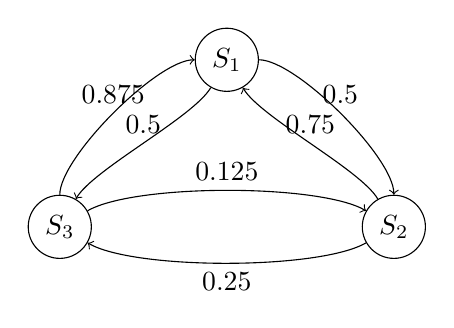
\begin{tikzpicture}[centered, node distance={30mm}, main/.style = {draw, circle}] 
\node[main] (1) {$S_1$}; 
\node[main] (2) [below right of=1] {$S_2$}; 
\node[main] (3) [below left of=1] {$S_3$}; 
\draw[->] (1) to [out=0, in=90, looseness=0.5] node[midway, above]{0.5} (2);
\draw[->] (1) to [out=240, in=60, looseness=0.5] node[midway, above]{0.5} (3);
\draw[->] (2) to [out=120, in=300, looseness=0.5] node[midway, above]{0.75} (1);
\draw[->] (2) to [out=210, in=330, looseness=0.5] node[midway, below]{0.25} (3);
\draw[->] (3) to [out=90, in=180, looseness=0.5] node[midway, above]{0.875} (1);
\draw[->] (3) to [out=30, in=150, looseness=0.5] node[midway, above]{0.125} (2);
\end{tikzpicture}
\end{center}

\section*{since $X$ is an irreducible markov chain that means it has a stationary distribution $\pi P = \pi$}

\begin{equation}
\begin{split}
& P = \begin{pmatrix}
0 & 0.5 & 0.5 \\
0.75 & 0 & 0.25 \\
0.875 & 0.125 & 0 \\
\end{pmatrix} 
\\
\\
& \begin{pmatrix}
\pi_1 & \pi_2 & \pi_3
\end{pmatrix}
*
\begin{pmatrix}
0 & 0.5 & 0.5 \\
0.75 & 0 & 0.25 \\
0.875 & 0.125 & 0 \\
\end{pmatrix}
= \begin{pmatrix}
\pi_1 & \pi_2 & \pi_3
\end{pmatrix} \\
& \begin{pmatrix}
0.75 \pi_2 + 0.875 \pi_3 \\
0.5 \pi_1 + 0.125 \pi_3 \\
0.5 \pi_1 + 0.25 \pi_2 \\
\end{pmatrix}
=
\begin{pmatrix}
\pi_1 \\
\pi_2 \\
\pi_3 \\
\end{pmatrix} \\
& \begin{pmatrix}
-\pi_1 + 0.75 \pi_2 + 0.875 \pi_3 \\
0.5 \pi_1 - \pi_2 + 0.125 \pi_3 \\
0.5 \pi_1 + 0.25 \pi_2 - \pi_3\\
\end{pmatrix}
=
\begin{pmatrix}
0 \\
0 \\
0 \\
\end{pmatrix} \\
& \begin{pmatrix}
-\pi_1 + 0.75 \pi_2 + 0.875 \pi_3 \\
\pi_1 - 2 \pi_2 + 0.25 \pi_3 \\
\pi_1 + 0.5 \pi_2 - 2 \pi_3 \\
\end{pmatrix}
=
\begin{pmatrix}
0 \\
0 \\
0 \\
\end{pmatrix} \\
& \begin{pmatrix}
-\pi_1 + 0.75 \pi_2 + 0.875 \pi_3 \\
- 1.25 \pi_2 + 1.125 \pi_3 \\
1.25 \pi_2 - 1.125 \pi_3 \\
\end{pmatrix}
=
\begin{pmatrix}
0 \\
0 \\
0 \\
\end{pmatrix} \\
& \begin{pmatrix}
-\pi_1 + 0.75 \pi_2 + 0.875 \pi_3 \\
- 1.25 \pi_2 + 1.125 \pi_3 \\
0 \\
\end{pmatrix}
=
\begin{pmatrix}
0 \\
0 \\
0 \\
\end{pmatrix} \\
& \text{but } \pi_1 + \pi_2 + \pi_3 = 1 \\
& \begin{pmatrix}
-\pi_1 + 0.75 \pi_2 + 0.875 \pi_3 \\
- 1.25 \pi_2 + 1.125 \pi_3 \\
0 \\
\pi_1 + \pi_2 + \pi_3 \\
\end{pmatrix}
=
\begin{pmatrix}
0 \\
0 \\
0 \\
1 \\
\end{pmatrix} \\
& \begin{pmatrix}
-\pi_1 + 0.75 \pi_2 + 0.875 \pi_3 \\
- 1.25 \pi_2 + 1.125 \pi_3 \\
0 \\
1.75 \pi_2 + 1.875 \pi_3 \\
\end{pmatrix}
=
\begin{pmatrix}
0 \\
0 \\
0 \\
1 \\
\end{pmatrix} \\
& \begin{pmatrix}
-\pi_1 + 0.75 \pi_2 + 0.875 \pi_3 \\
- 8.75 \pi_2 + 7.875 \pi_3 \\
0 \\
8.75 \pi_2 + 9.375 \pi_3 \\
\end{pmatrix}
=
\begin{pmatrix}
0 \\
0 \\
0 \\
5 \\
\end{pmatrix} \\
& \begin{pmatrix}
-\pi_1 + 0.75 \pi_2 + 0.875 \pi_3 \\
- 1.25 \pi_2 + 1.125 \pi_3 \\
0 \\
17.25 \pi_3 \\
\end{pmatrix}
=
\begin{pmatrix}
0 \\
0 \\
0 \\
5 \\
\end{pmatrix} \\
\end{split}
\end{equation}

\begin{equation}
\begin{split}
& \pi_3 = \frac{5}{17.25} = \frac{20}{69} \\
& -\frac{5}{4} \pi_2 + \frac{9}{8}\frac{20}{69} = 0 \\
& \pi_2 = \frac{20*9*4}{69*8*5}  = \frac{6}{23} \\
& -\pi_1 + \frac{3}{4}\frac{6}{23} + \frac{7}{8}\frac{20}{69} = 0 \\
& \pi_1 = \frac{9}{46} + \frac{35}{138} \\
& \pi_1 = \frac{27}{138} + \frac{35}{138} = \frac{62}{138} = \frac{31}{69}\\
& \pi = (\frac{31}{69}, \frac{6}{23}, \frac{20}{69})\\ 
\end{split}
\end{equation}

\section*{$\pi$ is the Markov chain's stationary distribution meaning it represents the proportion of time the flea spends at every vertex.}

\section*{Exercise 4.14. \normalfont Three people have a discussion about the upcoming elections. Everyone prefers one of two political parties, which we will abbreviate by V and W. We describe this by a Markov chain with four states $(S_0, S_1, S_2 \text{ and } S_3)$. In state $S_i$, W has i followers. If a faction has only one follower, then he has probability $\frac{1}{3}$ to convince another person to vote for that faction, while with probability $\frac{2}{3}$ he himself gets persuaded to vote for the other political party. As soon as everyone has the same opinion, the discussion ends. At time t = 0 the political party W has one follower.}

\section*{\normalfont (a) Draw the state diagram of this Markov chain, and give its transition matrix.}

\section*{Answer: }

\begin{center}
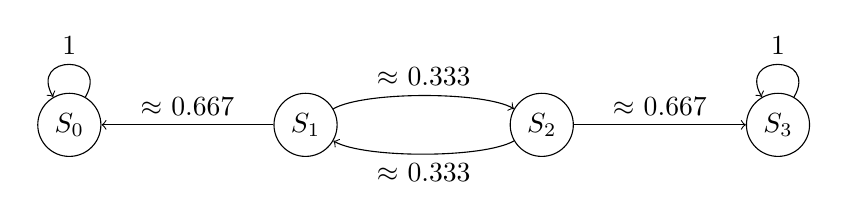
\begin{tikzpicture}[centered, node distance={30mm}, main/.style = {draw, circle}] 
\node[main] (0) {$S_0$}; 
\node[main] (1) [right of=0] {$S_1$}; 
\node[main] (2) [right of=1] {$S_2$}; 
\node[main] (3) [right of=2] {$S_3$}; 
\draw[->] (0) to [out=60, in=120, looseness=4] node[midway, above]{1} (0);
\draw[->] (1) to [out=180, in=0, looseness=0] node[midway, above]{$\approx$ 0.667} (0);
\draw[->] (1) to [out=30, in=150, looseness=0.5] node[midway, above]{$\approx$ 0.333} (2);
\draw[->] (2) to [out=210, in=330, looseness=0.5] node[midway, below]{$\approx$ 0.333} (1);
\draw[->] (2) to [out=0, in=180, looseness=0] node[midway, above]{$\approx$ 0.667} (3);
\draw[->] (3) to [out=60, in=120, looseness=4] node[midway, above]{1} (3);
\end{tikzpicture}
\end{center}

\begin{equation}
P = \begin{pmatrix}
1 & 0 & 0 & 0 \\
\frac{2}{3} & 0 & \frac{1}{3} & 0 \\
0 & \frac{1}{3} & 0 & \frac{2}{3} \\
0 & 0 & 0 & 1 \\
\end{pmatrix}
\end{equation}

\section*{\normalfont (b) Give the probability distribution at t = 3.}

\section*{Answer: The probability distribution at time t = 3 is dependant on the initial distribution. Since the initial distribution isn't given the resulting distribution will be a function of the initial distribution.}

\begin{table}[ht]
\centering
\begin{adjustbox}{width=1\linewidth}
\begin{tabular}{c|cccc}
 & t = 0 & t = 1 & t = 2 & t = 3\\ \hline
$S_0$ & $\pi_0$ & $\pi_0 + \frac{2}{3}\pi_1$ & $\pi_0 + \frac{2}{3}\pi_1 + \frac{2}{9}\pi_2$ & $\pi_0 + \frac{20}{27}\pi_1 + \frac{2}{9}\pi_2$\\ 
$S_1$ & $\pi_1$ & $\frac{1}{3}\pi_2$ & $\frac{1}{9}\pi_1$ & $\frac{1}{27}\pi_2$ \\ 
$S_2$ & $\pi_2$ & $\frac{1}{3}\pi_1$ & $\frac{1}{9}\pi_2$ & $\frac{1}{27}\pi_1$ \\ 
$S_3$ & $\pi_3$ & $\pi_3 + \frac{2}{3}\pi_2$ & $\pi_3 + \frac{2}{3}\pi_2 + \frac{2}{9} \pi_1$ & $\pi_3 + \frac{20}{27}\pi_2 + \frac{2}{9}\pi_1$ \\ 
\end{tabular}
\end{adjustbox}
\caption{Visualization of P(T|C). } 
\end{table}

\section*{\normalfont (c) Which of the states are absorbing?}

\section*{Answer: Absorbing state is a state which once entered cannot be left, in this case the state $S_i$ has $P_{ii}^{(t)} = 1$, meaning once entered in can only stay in $S_i$. In this case those would be the states $S_0, S_3$.}

\section*{\normalfont (d) What is the probability to eventually end in state $S_3$?}

\section*{Answer: Since $\{S_3\}$ is a closed class that means that once we enter we cannot leave so all we need to do is calculate the probability from each state that we enter $S_3$ once.}

\begin{equation}
\begin{split}
h_{0,3} & = 0 \text{ since $S_0$ is closed} \\    
h_{1,3} & = \frac{2}{3} h_{0,3} + \frac{1}{3} h_{2,3} \\
h_{2,3} & = \frac{2}{3} h_{3,3} + \frac{1}{3} h_{1,3} \\
h_{3,3} & = 1 \\
h_{1,3} & = \frac{1}{3} h_{2,3} \\
h_{2,3} & = \frac{2}{3} + \frac{1}{3} h_{1,3} \\
h_{2,3} & = \frac{2}{3} + \frac{1}{9} h_{2,3} \\
\frac{8}{9} h_{2,3} & = \frac{2}{3} \\
h_{2,3} & = \frac{3}{4} \\
h_{1,3} & = \frac{1}{3} \frac{3}{4} \\
h_{1,3} & = \frac{1}{4} \\
\text{All of these probabilities } & \text{assume we start at that state.} \\
\text{The total probability is } & \text{the weighted sum with the initial distribution.} \\
P(\text{ending in } S_3) & = \pi_0 h_{0,3} + \pi_1 h_{1,3} + \pi_2 h_{2,3} + \pi_3 h_{3,3} = \\ 
& =\frac{1}{4} \pi_1 + \frac{3}{4} \pi_2 + \pi_3 \\
\end{split}
\end{equation}
Something that should be noted is that this probability is entirely dependent on the initial distribution since the Markov chain is reducible. So without an initial distribution, an exact answer cannot be given.

\end{document}
